\RequirePackage[l2tabu, orthodox]{nag}

\documentclass[10pt]{scrartcl}
\usepackage[T1]{fontenc}
\usepackage{amsmath,amsfonts,amssymb}
\usepackage{mathtools}
\usepackage{cancel}
\usepackage{color,soul}
\usepackage[margin=2cm,letterpaper]{geometry}
\usepackage{enumerate}
\usepackage{graphicx}
\usepackage[colorlinks=true,urlcolor=blue]{hyperref}
\usepackage{floatrow}
\usepackage{deluxetable}
\usepackage{verbatim}
\usepackage{fancyvrb}
\usepackage{listings}
\usepackage{calc}
\usepackage{xfrac}
\usepackage{cleveref}
\usepackage[font=small]{caption}
\usepackage[font=scriptsize]{subcaption}
\usepackage[activate={true,nocompatibility},final,tracking=true,kerning=true,spacing=true,factor=1100,stretch=10,shrink=10]{microtype}
\SetTracking{encoding={*}, shape=sc}{40}

\microtypecontext{spacing=nonfrench}

\floatsetup{ 
  heightadjust=object,
  valign=t
}

\definecolor{Light}{gray}{.90}
\sethlcolor{Light}

\lstset{%
language=IDL,                       % choose the language of the code
basicstyle=\footnotesize\sffamily,  % the size of the fonts that are used for the code
numbers=left,                       % where to put the line-numbers
numberstyle=\footnotesize,          % the size of the fonts that are used for the line-numbers
stepnumber=1,                       % the step between two line-numbers. If it is 1 each line will be numbered
numbersep=5pt,                      % how far the line-numbers are from the code
showspaces=false,                   % show spaces adding particular underscores
showstringspaces=false,             % underline spaces within strings
showtabs=false,                     % show tabs within strings adding particular underscores
frame=single,                       % adds a frame around the code
backgroundcolor=\color{Light},
columns=flexible,
tabsize=2,                          % sets default tabsize to 2 spaces
captionpos=b,                       % sets the caption-position to bottom
breaklines=true,                    % sets automatic line breaking
breakatwhitespace=false,            % sets if automatic breaks should only happen at whitespace
escapeinside={\%*}{*)}              % if you want to add a comment within your code
}

\title{Why We Do What We Do (WWDWWD)}
\author{Jeren Suzuki}
\date{Last Edited \today}

\begin{document}

\pagenumbering{gobble}
\maketitle
\tableofcontents
\addcontentsline{toc}{section}{Introduction}
\clearpage
\pagenumbering{arabic}

\section*{Introduction} % (fold)
\label{sec:introduction}
\indent This document is an attempt to organize the decision behind our methods in the grand scheme plan of extracting useful data from our image. I will try to organize it in parts so that it will be easier to follow.
% section introduction (end)

\section{Data Acquisition} % (fold)
\label{sec:data_acquisition}
Even before we have an image, we have to talk to the camera, so to speak. This involves installing the PvPAPI SDK on an Ubuntu machine, connecting the machine directly to the camera through an ethernet port, then manually setting the network interface to lie on the same subnet as the camera (the camera has a static IP address so it must be done on the computer). Once the IP address and subnet mask (and gateway too?) are configured correctly, the camera can be set to take pictures by navigating to the \texttt{AVT GiGE SDK} $\rightarrow$ \texttt{bin-pc} $\rightarrow$ \texttt{x64} directory and running \texttt{SampleViewer}. You should see a widget appear with the camera listed in the interface. Setting up the camera is beyond the scope of this document but I have partial instructions in \texttt{sdkrefman} and Nicole has printed out instructions in one of her binders. 

\subsection{Setting up image} % (fold)
\label{sub:setting_up_image}

Now that we've setup the camera, we need something to take pictures of. We simulate a solar image based on the images we received from Albert. To do this, we need:

\begin{itemize}
    \item Pixel pitch of camera sensor (physical size of pixel)\\   
        If you don't have the pixel pitch, use the physical sensor dimensions against the image resolution
    \item Distance from focal plane to imaged plane
    \item Focal length of lens
\end{itemize}

we stick them into this equation:

\begin{equation}
    \frac{\textrm{pixel pitch}}{\textrm{focal length}} = \frac{\textrm{physical length of a pixel in the image}}{\textrm{Distance from focal plane to imaged plane}-\textrm{focal length}}
\end{equation}

If we want the sun to be $N$ pixels wide (corresponding to $M$ cm), then open an image editor at 300 pixels/cm and make a sun 

\begin{align}
    300 ~\frac{\textrm{pixels}}{\textrm{cm}} \cdot M ~\textrm{cm}\\
    300 ~\frac{\textrm{pixels}}{\cancel{\textrm{cm}}} \cdot M ~\cancel{\textrm{cm}}\\
    300 \cdot M~\textrm{pixels wide}
\end{align}

\Cref{ohyeah} compares the \emph{fiducials} we were testing to the starting image we based them off. \emph{Fiducials}. Not the shape/size of the sun.

\begin{figure}[!ht]
    \ffigbox[][\FBheight]{%
    \begin{subfloatrow}[2]%
        \ffigbox[\FBwidth]%
       {%
       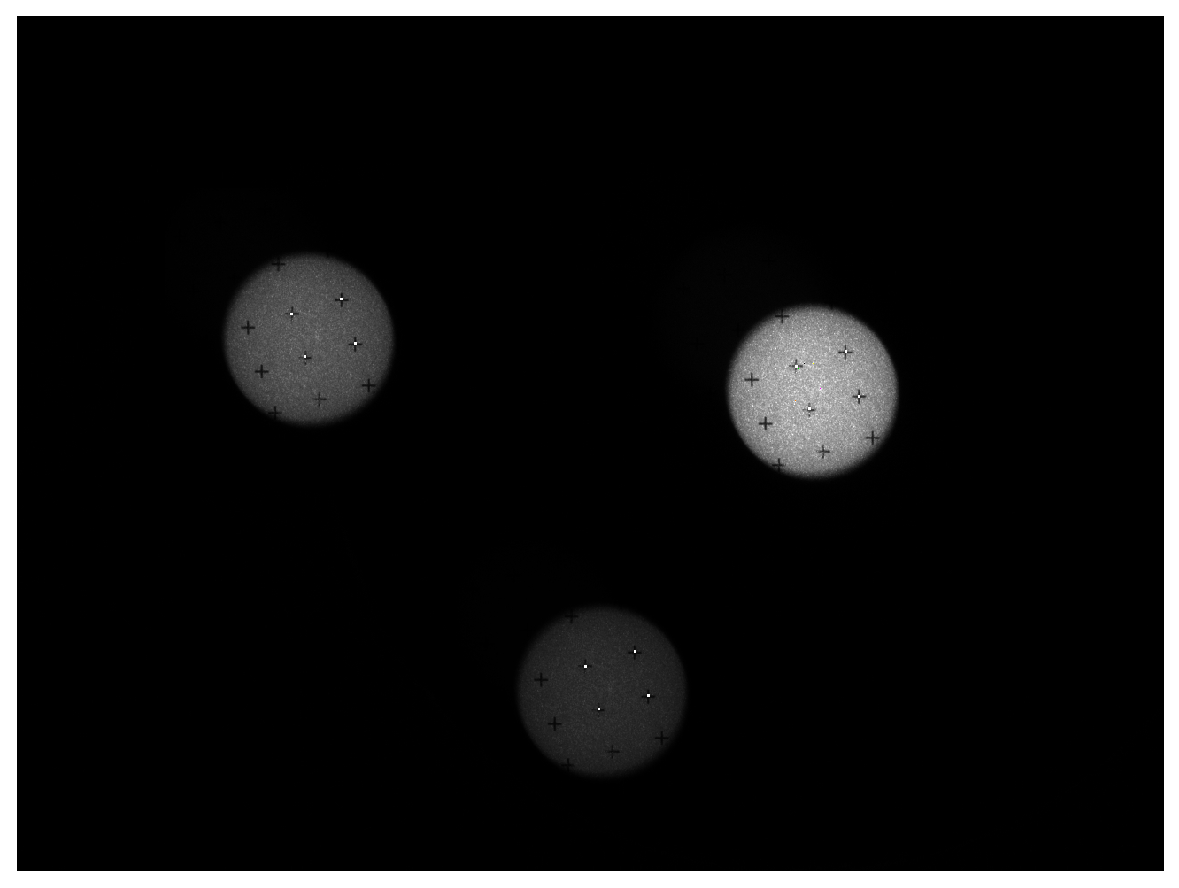
\includegraphics[width=.5\textwidth]{../plots_tables_images/best4_actual.eps}%
       }%
       {%
       \caption{The image we based the fiducial dimensions on (and only fiducial dimensions, not solar dimensions)}%
       }%
        \ffigbox[\Xhsize]%
       {%
       \includegraphics[width=.5\textwidth]{../plots_tables_images/best4.eps}%
       }%
       {%
       \caption{Our simulated image. Ignore the hilariously large sun and notice the fiducials are about the same size.}%
       }%
    \end{subfloatrow}}{\caption{}\label{ohyeah}}%
\end{figure}

% subsection setting_up_image (end)
% section data_acquisition (end)

\section{Handling The 2D Image} % (fold)
\label{sec:handling_the_2d_image}

\subsection{File Formats} % (fold)
\label{sub:file_formats}
In an effort to maintain maximum portability across all platforms, we saved all our images in the \emph{FITS} file format. Any images received for testing purposes (for example, the ones from Albert), I opened in IDL and converted into FITS. 

\subsubsection{Specific to Photos from a DLSR} % (fold)
 \label{ssub:specific_to_photos_from_a_dlsr}
When dealing with images generated with my DLSR when taking bundle mask images, they had to be converted from RAW into 16 bit TIFF, then loaded into IDL. JPEG files introduced artifacts and the actual range of a pixel in a JPEG file wasn't as high. TIFF files were considered filled with unsigned integers while JPEG files only ranged in byte values. If there is the option, use TIFF files. The only problem is that TIFF files are incredibly large.  

Also, photos taken from my camera come with three channels, red, green, and blue. When doing image analysis, I chose the image with the most contrast when on a black-white color table. The fits files contain the first channel of the 3 channel image (the red channel) when loaded with either \hl{\texttt{READ\_JPEG}} or \hl{\texttt{READ\_TIFF}}.
% subsubsection specific_to_photos_from_a_dlsr (end) 
% subsection file_formats (end)

\subsection{Finding Region Number} % (fold)
\label{sub:finding_region_number}
The current method of determining which brightness suns are in the image involves matching up appropriate pixel values to threshold values. If we have 2 suns, we can't determine which brightness suns we have without actually looking at the brightness values. We ended up partitioning the brightness into three regions: < 30\%, > 60\%, and between 30\% and 60\%. Then, we look at however many suns are in our image and look at the max value in each sun. Whatever region the max pixel falls under, the entire sun is marked with that region number. This way, we can correctly determine an image with a region 1 and 3 run (brightest sun and 25\% brightness sun). 

A problem with this method is that I have to use IDL's \hl{\texttt{LABEL\_REGION}} and \hl{\texttt{HISTOGRAM}} function. These are not exactly trivial and easy-to-build-from-scratch functions that we can port into \texttt{C++}, so we need to either think of a different solar region identification method or find a simpler way to do it. 

One of \hl{\texttt{LABEL\_REGION}}'s strengths is that any adjacent pixels in a mask count towards a single region number. The downside is that isolated pixels are also treated as individual regions. There are two ways to fix this. One is to use the \hl{\texttt{DILATE}} function to expand stray pixels to overlap with nearby blobs (the technical term), creating a contiguous chunk. The other method is simply let \hl{\texttt{LABEL\_REGION}} do it's work and apply region numbers to everything, no matter how many pixels are contiguous. Then, we tell \hl{\texttt{HISTOGRAM}} to only analyze blobs with pixel counts greater than, say, 1000. In the end, we chose the former method.
% subsection finding_region_number (end)

% section handling_the_2d_image (end)

\section{Skimming the Top Off} % (fold)
\label{sec:skimming_the_top_off}
We want to eliminate any outlier pixels that are too bright so we sort our 2D image as a 1D array and remove the top 1\% (or .1\%, whatever) of the pixels for our threshold. Even though in the sample images provided by Albert there are no bright outlier pixels, eliminating the brightest pixels poses no detrimental affect to image processing. The reason why we do this is because having abnormally large values messes up the 2nd derivative for threshold-setting.
% section skimming_the_top_off (end)

\section{Deciding Whether or Not to Keep Image} % (fold)
\label{sec:deciding_whether_or_not_to_keep_image}
The two methods we moved past:

\begin{enumerate}
    \item Check for bright pixels on image border, if number of continuous bright pixels exceeds a threshold, the general area is considered ``\emph{bad}''
    \item Count bright pixels on image border mask, if number exceeds a certain threshold, use further processing to determine where in the image the bad sun lies
\end{enumerate}

To make sure that we identify the appropriate centers of the sun, we have to know how many are actually in the picture. First, we check if there are any pixels on the border of the image that are a significantly higher value than the mode of the image. If we see $N$ pixels on the border, then one of the suns is cut off. If we see $N$ and $Z$ pixels on the border, then we take into account 2 cut-off suns. We make sure that if we see no sun-pixels on the border that there isn't a chance that we missed a sun altogether and there are only 2 suns in the image. 

\begin{figure}[!ht]
    \ffigbox[][\FBheight]{%
    \begin{subfloatrow}[2]%
        \ffigbox[\FBwidth]%
       {%
       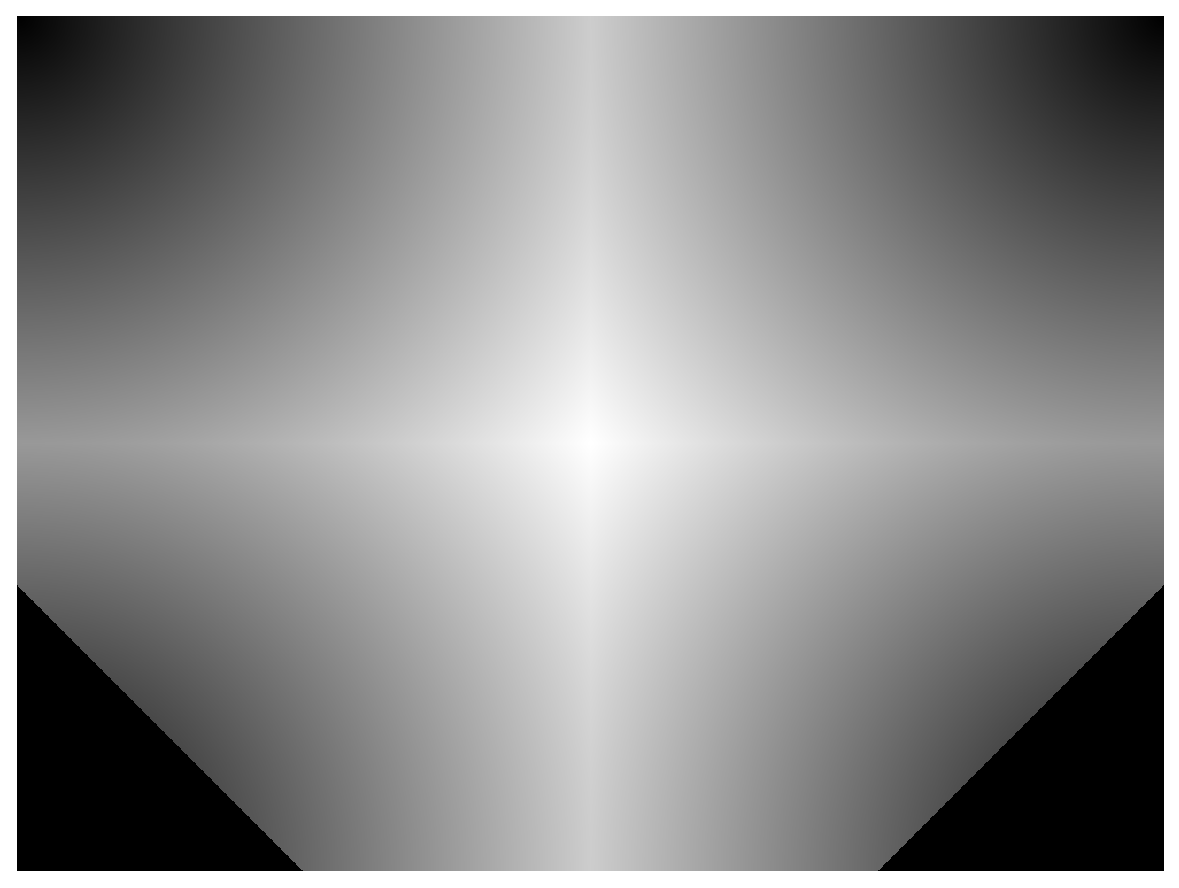
\includegraphics[width=.5\textwidth]{../plots_tables_images/distmask.eps}%
       }%
       {%
       \caption{The image mask with the bottom corners as no-data zones}%
       }%
        \ffigbox[\Xhsize]%
       {%
       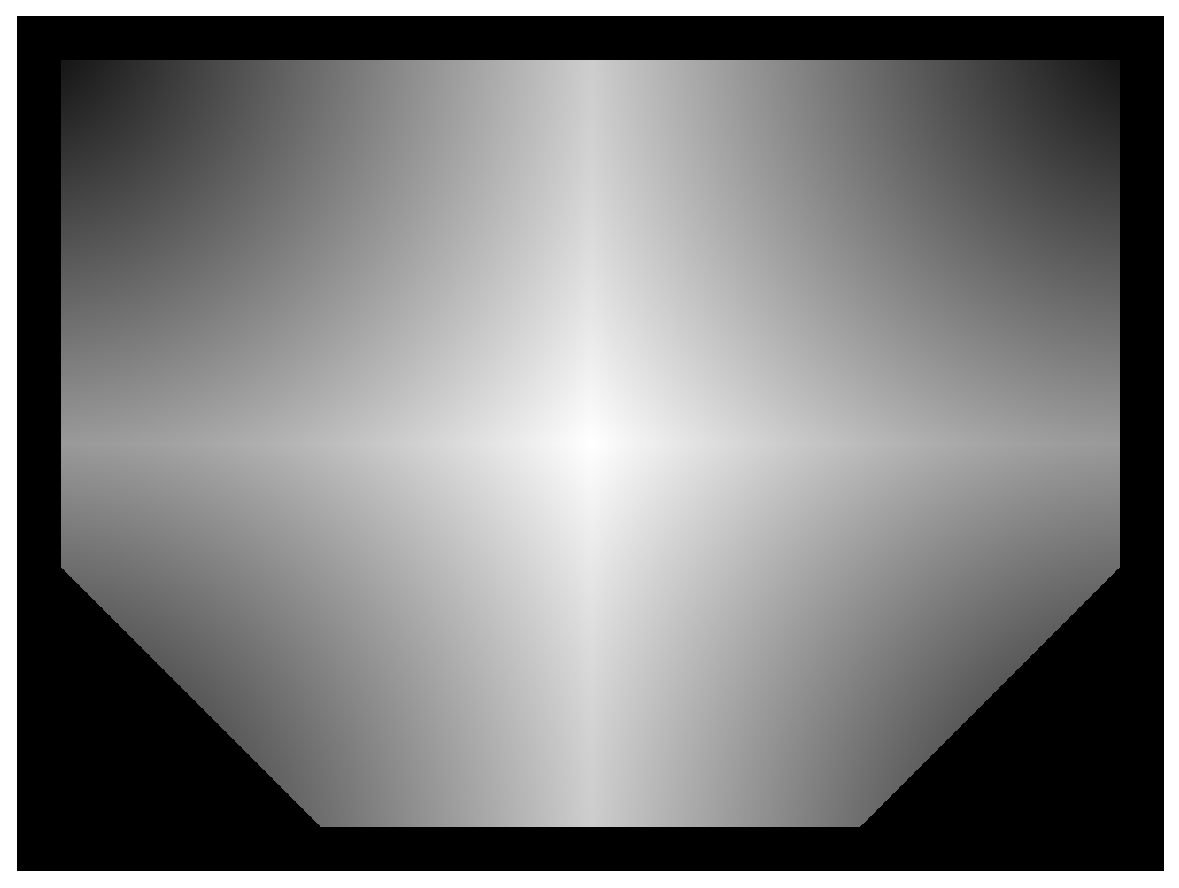
\includegraphics[width=.5\textwidth]{../plots_tables_images/distfixedmask.eps}%
       }%
       {%
       \caption{What the initial attempts at border-masking achieved, although at the heavy cost of time. If there were any solar pixels identified in that border region, then further processing would occur.}%
       }%
    \end{subfloatrow}}{\caption{}\label{corner}}%
\end{figure}

A border mask is easy to construct for a rectangle, but when you start throwing in angles, the amount of time it takes to construct the mask increases quickly. (To see what a border mask looks like, see \cref{corner}) To deal with the bottom two corners, which are areas which will never see any data, one method was to make triangular matrices with 0s and 1s and then append them to the bottom corners of a large rectangular matrix. Another method was to use \hl{\texttt{shift}} to move around the rectangular matrix within a larger matrix, multiply the shifted matrices together, and then crop the final matrix down to the original size. Both this method and the counting pixels method were slow, however. \\

We ended up with a 2-part check that uses coordinate transformation. First, we check if the solar center is within a certain distance to the edge. Next, we rotate the coordinates of the center by 45$^\circ$ and check how lose it is to the edge of the image (or whatever bounds we want). This essentially lets us quickly map out the bottom corners. See \cref{cchecks}.

\begin{figure}[!ht]
    \ffigbox[][\FBheight]{%
    \begin{subfloatrow}[2]%
        \ffigbox[\FBwidth]%
       {%
       \includegraphics[width=.5\textwidth]{../plots_tables_images/firstcheck.eps}%
       }%
       {%
       \caption{The gray square simulates the solar image with 3 suns. The black dot is the center of a sun that would otherwise be considered ``good'' by the program since it doesn't take into account the bottom corners.}%
       }%
        \ffigbox[\Xhsize]%
       {%
       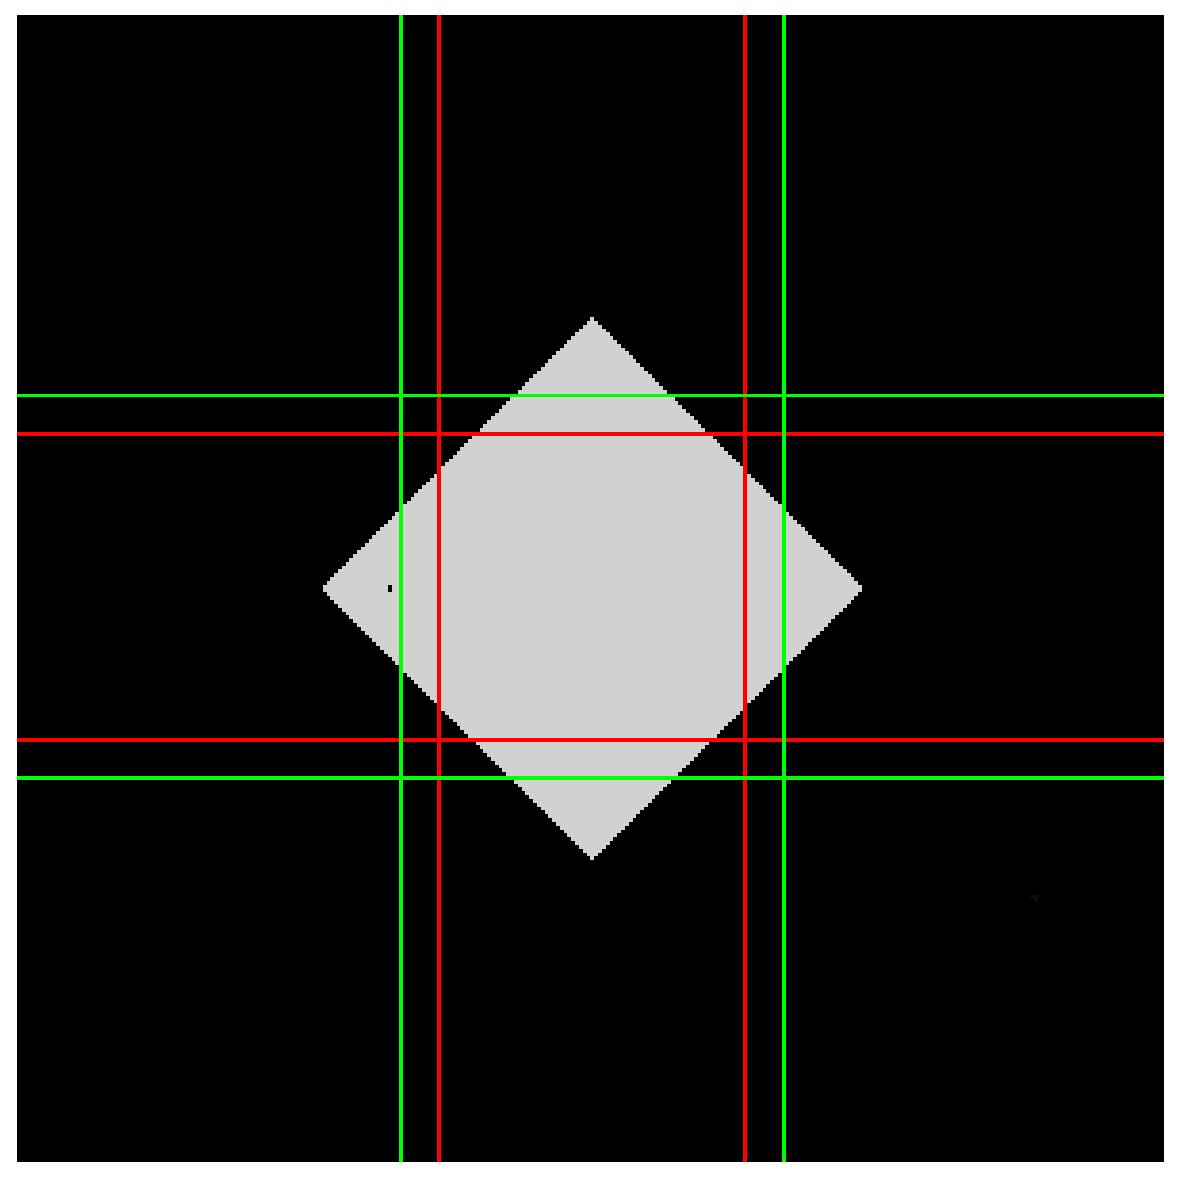
\includegraphics[width=.5\textwidth]{../plots_tables_images/seccheck.eps}%
       }%
       {%
       \caption{With the image rotated 45$^\circ$ (but in reality, only the black dot is rotated. the entire array is rotated here to show the effect), the black dot now lies beyond the green line, which is the original border of the gray square. The left vertical and bottom horizontal green line mark the boundary regions for the bottom two corners. This method is fast.}%
       }%
    \end{subfloatrow}}{\caption{}\label{cchecks}}%
\end{figure}

% section deciding_whether_or_not_to_keep_image (end)

\section{Finding Centers of Sun(s)} % (fold)
\label{sec:finding_centers_of_sun}

Our mask centroiding program takes the center of mass of any shape above a certain threshold. We then zero-out a box around the sun, and find the center of mass of the next shape above a threshold. 

There was another method we didn't get very far on, but it had the potential to being a lot faster and \emph{maybe} more robust. We sorted the 2D image instead of by value, but by either x or y position. In \cref{sortsort}, the top image is the 2D sorted image by x position. The three sideways finger shapes correspond to the three solar regions. The very dark tips seem to end where the other begins (in the x-axis). With the first threshold (which is defined by a vertical line and anything to the right of the line is considered above the threshold), we eliminate the rightmost finger thing by zeroing out anything a little before and after the x range of the pixels, leading to the second row. This puts the second brightest sun as the rightmost finger. Process is repeated until all suns have been cropped. This method is faster because it doesn't deal with the re-processing of a 2D image, instead it zeroes out indices in a 1D array (or even faster, looks elsewhere in the array and doesn't reindex anything).

This method was tested because it reused the \hl{\texttt{sort()}} function when making the threshold and simply applied the sort indices to x and y positions instead of pixel values. The result was a fast and robust centering method. The problem was if the suns lied in either the x or y axes (which is most probably the case). As you can see from the figure, if any of the suns share the same x or y range, even a little bit, the centering will be off (See \cref{sortsortohno}). A solution was to check both the x and y indices (because you can't overlap in both), but further development was stopped in favor of a more intuitive (and easier to code) approach. I think we could've made it work though.\\

% \begin{figure}[!ht]
%    \includegraphics[width=\textwidth]{../plots_tables_images/quickcenters.png}%
%    \caption{The 2D array sorted by x or y positions}\label{sortsort}
% \end{figure}

\begin{figure}[!ht]
    \ffigbox[][\FBheight]{%
    \begin{subfloatrow}[2]%
        \ffigbox[\FBwidth]%
       {%
       \includegraphics[width=.5\textwidth]{../plots_tables_images/quickcenters.png}%
       }%
       {%
       \caption{The 2D array sorted by x or y positions}%
       \label{sortsort}%
       }%
        \ffigbox[\Xhsize]%
       {%
       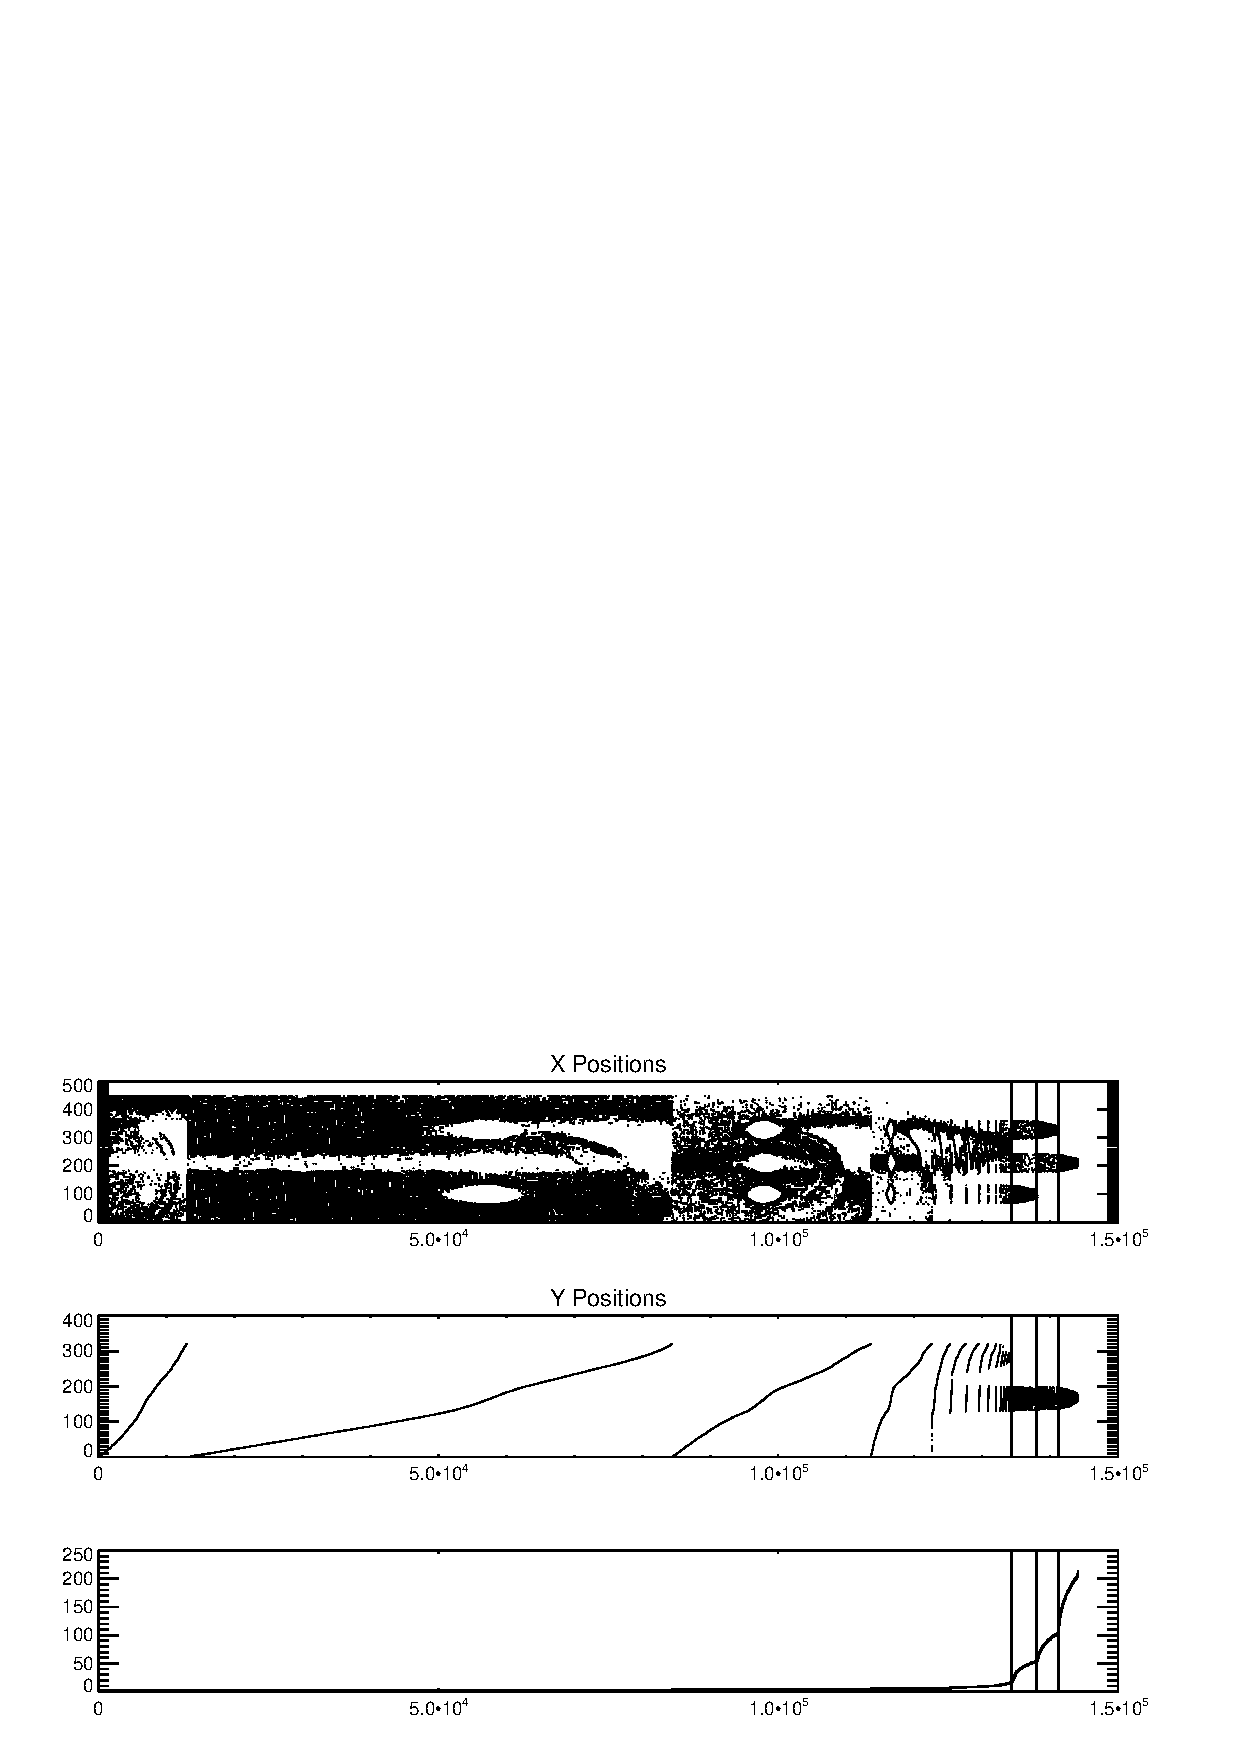
\includegraphics[width=.5\textwidth]{../plots_tables_images/inaline.png}%
       }%
       {%
       \caption{Here, the suns are lined horizontally so all the y positions overlap. If we zero out the y range a little before and after the pixels to the right of the rightmost vertical line in the `Y Positions' plot, we end up zeroing out the y range of the other suns too.}%
       \label{sortsortohno}%
       }%
    \end{subfloatrow}}{\caption{}}%
\end{figure}

Once we find the approximate centers, we crop a box around the sun and create arrays the entire length of the cropped box. Next, we isolate and limb fit the edges of the sun so that we can find more accurate center positions. At first we used a 3 order fit, then a linear fit (since that's what Albert used), then to a 2nd order fit (because we thought it wasn't good enough) then back to a linear fit (because the fit was good enough). 

\subsection{Thresholds} % (fold)
\label{sub:thresholds}
We want a robust threshold so instead of using an arbitrary parameter multiplied by the max of the image, we sort the 2D image into a 1D array and return the position of the boundaries of the regions which are seen as humps. See \cref{peaks}.

To find the boundaries, we look at the 2nd derivative of the sorted array and find the 3 maximum peaks (in the case of 3 suns), corresponding to the boundaries of the aforementioned humps. We chose this way because thresholding the peaks requires parameterization that needs to be changed dynamically. 

\begin{figure}[!ht]
   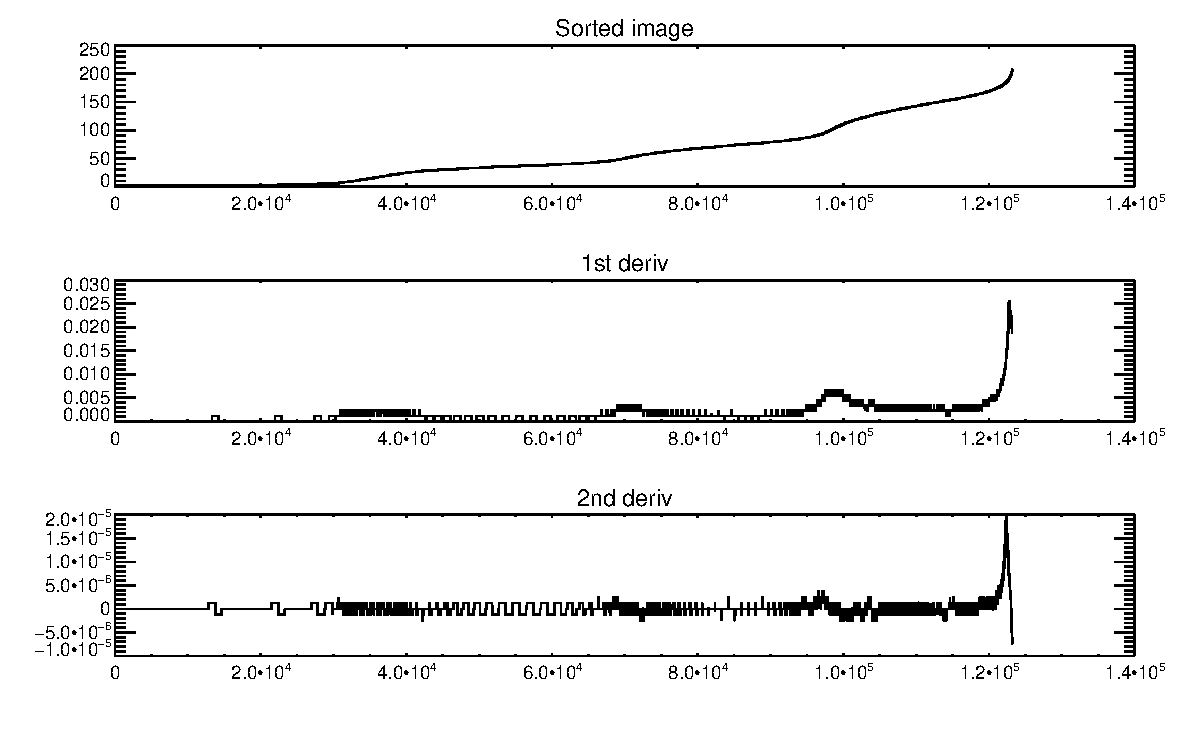
\includegraphics[width=.75\textwidth]{../plots_tables_images/sortedarray.eps}%
   \caption{This is the sorted array for a 3-sun image. The peaks don't look that large in the second derivative, but that's just because of the scaling to the first peak.}\label{peaks}
\end{figure}

Several factors affecting thresholding values:

\begin{enumerate}
    \item \hl{\texttt{smooth()}} parameters
    \item unusually bright pixels
    \item artifacts of smoothing
\end{enumerate}

To solve 1), we used the \hl{\texttt{edge\_truncate}} keyword because it gave us the least amount of weird edge artifacts in the 1D array. The other options were \hl{\texttt{edge\_zero}} and \hl{\texttt{edge\_mirror}} which yielded poor results.

To solve 2), when we sorted the array by brightness, we left out the top .1\% of the pixels.

To solve 3), we had to manually cut off the last 10,000 pixels. This part needs to be improved.

Since we knew there were approximately $N$ pixels per sun, we looked into partitioning the 1D sorted array into chunks with $N$ pixels to calculate the threshold from. Not sure why we stopped this, but it was for a good reason.
% subsection thresholds (end)
% section finding_centers_of_sun (end)

\section{Finding Fiducial Positions} % (fold)
\label{sec:finding_fiducial_positions}

Now that we have a limb-fitted centroid, we analyze the sun for fiducials. They are characteristically dark, so we ended up looking at 1D sums in the row/column directions and looking for dips in brightness (where 1D sums line up with the entire length of the fiducial). Before this method, we looked at a few other options. They included:

\begin{enumerate}
    \item Running edge detector filters to isolate the edge of the fiducials
    \item Applying convolution/cross-correlation filters 
\end{enumerate}

For edge detection filters, we looked at \hl{\texttt{emboss}}, \hl{\texttt{shift\_diff}}, and \hl{\texttt{laplacian}}. Using 2D filters posed a few problems. One, it was time consuming because it required processing on a 2D array. Two, the result was a 2D array that we had to further process. Depending on how high we set our threshold we would either get too little or too many pixels to judge where the fiducial edge was. If there were too many pixels, we count each row/column and take the row/column with more pixels thresholded to be the fiducial row/column. This is seen in \cref{edge_det}. The pixels outlined are above a certain threshold  but there is obviously one row/col with a fiducial.\\

The basics of edge detection filters was that when we run them with a kernel that emphasized an edge of the fiducial, we get an array that traces out the shape of the fiducial (to some extent). For the case of \hl{\texttt{shift\_diff}}, a high value corresponds to a leading edge and a low value to a falling edge. We threshold the 2D image for a high threshold so we retrieve all the leading edges in a certain direction. Next, we see where in the image the leading edges are so that we can pinpoint exact fiducial positions. An immediate downside of this method is that the fiducals must be lined up vertically and horizontally or be offset enough that no two fiducials share the same row/column \emph{range} for this to work. Also, if the image is rotated more than 5 degrees (which according to Nicole, shouldn't happen), then incorrect fiducial positions are returned. This is so that when one fiducial ends, some other fiducial's limb won't overlap.

\begin{figure}[!ht]
   \includegraphics[width=.75\textwidth]{../plots_tables_images/threshtesh_3.png}%
   \caption{The pixels outlined correspond to values from the edge detection-filtered array}\label{edge_det}
\end{figure}

Another problem with edge detection was that it returned the x and y positions of each fiducial candidate in no specific order. They weren't paired up in any way so we got a long list of x and y positions and had to look at each possible fiducial pair and determine if there was actually a fiducial there or not. First, we checked to see if the fiducial coordinate was more than a certain distance from the solar center (because we only care about fiducials close to the center anyhow). The, we checked if the pixel value at the coordinate dim enough. Once it passed this second check, we cropped a small area around the fiducial candidate and looked at the 1D sums per row/column. If there is a dip in both directions (characteristic of a fiducial), then the fiducial candidate is confirmed as an actual fiducial.\\

In addition to using edge detection filters to find fiducials, we also looked at a convolution/cross correlation filter. I mention cross correlation because it is the method Albert used in his image analysis code. Convolution and edge detection filters only differ by the shape and content of the kernel so it required many a tweaks to find one that emphasized the shape of the fiducial while suppressing foreign noise and shapes. \Cref{cropcomp} illustrates an example of a convolution filter output.

% \begin{figure}[!ht]
%    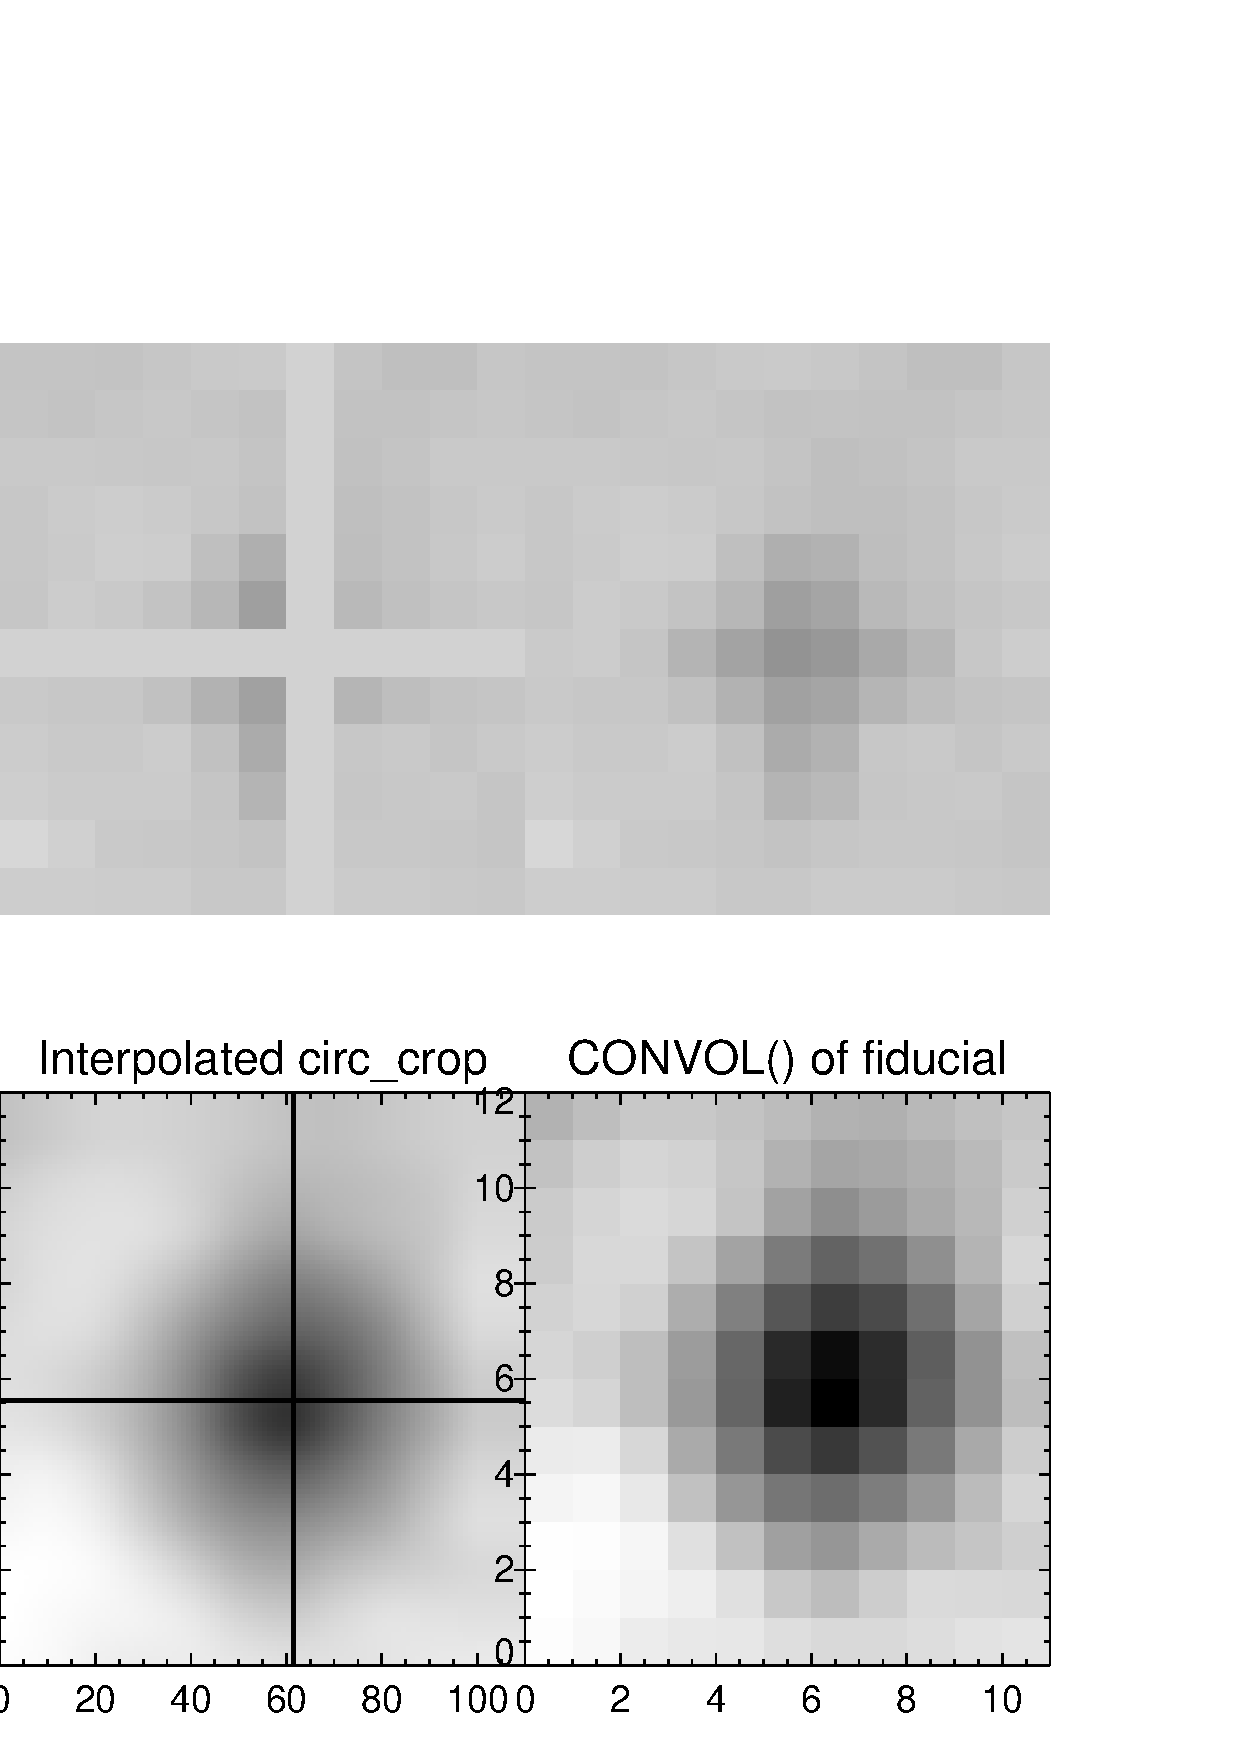
\includegraphics[width=.5\textwidth]{../plots_tables_images/cropcomp3.png}%
%    \caption{Result of convolution filter designed to create a blurry minimum.}\label{cropcomp}
% \end{figure}

\begin{figure}[!ht]
    \ffigbox[][\FBheight]{%
    \begin{subfloatrow}[2]%
        \ffigbox[\FBwidth]%
       {%
       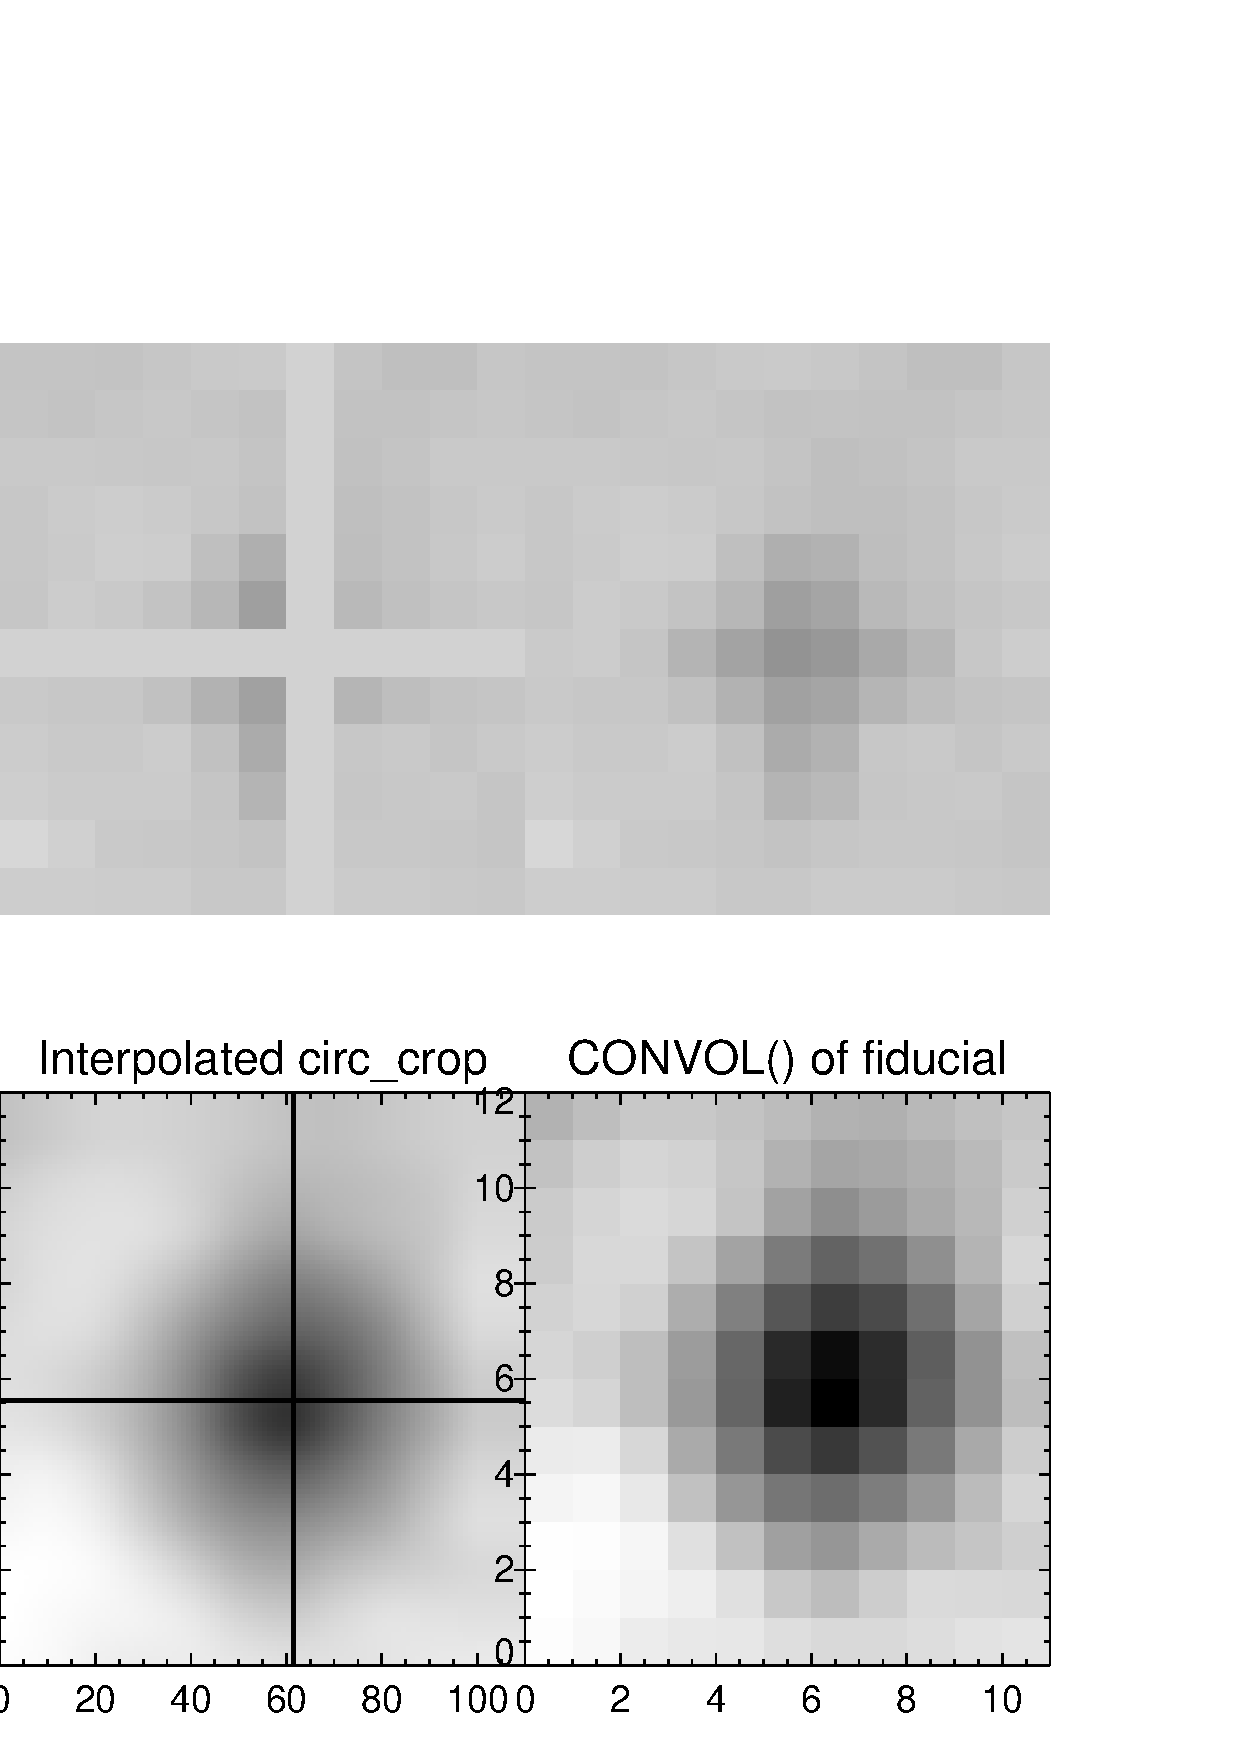
\includegraphics[width=.5\textwidth]{../plots_tables_images/cropcomp3.png}%
       }%
       {%
       \caption{Result of convolution filter designed to create a blurry minimum.}%
       \label{cropcomp}%
       }%
        \ffigbox[\Xhsize]%
       {%
       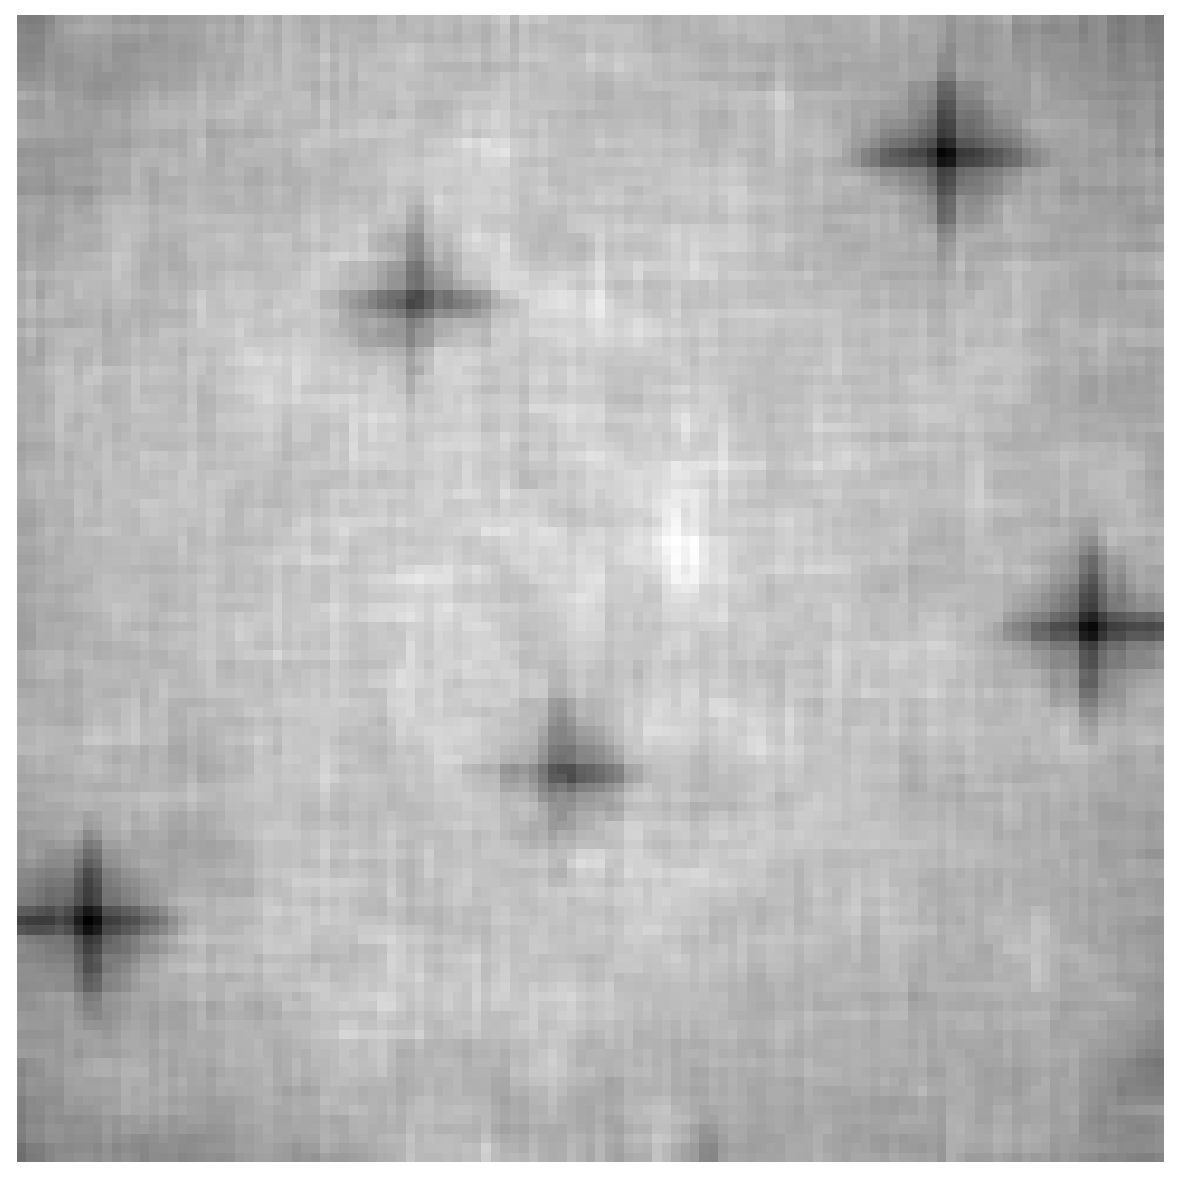
\includegraphics[width=.5\textwidth]{../plots_tables_images/sharpfid.eps}%
       }%
       {%
       \caption{Using a kernel that emphasized a sharp peak instead of a smooth minimum.}%
       \label{sharpfid}%
       }%
    \end{subfloatrow}}{\caption{}}%
\end{figure}


There were two options for kernel design, one was to make a blurred out smooth local minima with a minimum at the fiducial center and the other was a sharp extended plus shape that had a very high center value (See \cref{sharpfid}). The blurred out smooth minimum ended up finding a more consistent fiducial center even though to our eyes, the sharp result from the extended plus shape seemed more accurate. The strength of the convolution filter was that the fiducials could be in any position or orientation, the filter didn't care. We were finding the centers of the fiducials by looping through the array and checking for a local minimum. \\

Another problem related to fiducial finding is dealing with fiducials on the edge of the sun. If a fiducial lies on the edge, it is hard to distinguish from the edge pixels without some sort of spatial information, like a convolution filter. We came up with a bunch of methods for dealing with edge fiducials but since the only fiducials we care about are near disk-center, we can just ignore the fiducials too far out. The number of fiducials we look at close to disk-center (4) is arbitrary; it should probably depend on the density of fiducials on the plane. 

\subsection{Subpixel Fiducial Positions} % (fold)
\label{sub:subpixel_fiducial_positions}
All the aforementioned methods deal with how to get fiducials positions to pixel-level accuracy. We could interpolate the 2D convolution filter output to achieve subpixel values but we'd be adding data instead of fitting to data we already have. A solution is using 2 1D parabolic fits. This method is applied on the 1D sums; once we find fiducials in our program, we crop a smaller box surrounding the fiducial and calculate the 1D sums in both directions. A characteristic dip forms, and we fit a 3 pixel range straddling the 1D sum minimum and fit a parabola to it. We do this in the other direction and then calculate where the two parabolas intersect. This method is fast because it doesn't call any external fitting functions and is just algebra.  
% subsection subpixel_fiducial_positions (end)

% section finding_fiducial_positions (end)

\section{Fiducial Identification} % (fold)
\label{sec:fiducial_identification}
This part of the code is still incomplete but I will attempt to address the methods used. Towards the end of our program we've isolated the 4 closest fiducials to the center of a given sun. Now, we have to identify which fiducials are which. One way to do this is to look at the distances between fiducials and match them up that way. We construct an irregular grid so that no two distances between fiducials are the same. So. We have 4 fiducials, so there are 6 (4 choose 2) possible distance combinations between the fiducials. We have a long catalog of distances that we match up our 6 numbers against to find out which fiducials are being counted for. Every distance, however, links to a pair of fiducials so we have to determine which fiducial is which within a pair. 

We can do this by having an array 4 elements long, one for each fiducial. Starting at one fiducial, we look at all possible distances combinations. Let's say we start from the $A$ fiducial, so we care about $\overline{AB},\overline{AC},$ and $\overline{AD}$. We look up in the table these distances and for each matched pair, we add a marker to the 4 element matrix for the \emph{real} fiducial tags they contain. Our A through D naming system is just a placeholder until we can correctly identify the fiducials. Let's say we look at $\overline{AB}$ and find that in our catalog, that distance corresponds to the distance from F2 to F4. In our array, we mark:

\begin{align}
  &[\texttt{F1,F2,F3,F4}]\\
  &[\texttt{0 ,1 ,0 ,1 }]~,\textrm{The fiducial connects these two points}
\end{align}

Then, we look at the next distance segment, $\overline{AC}$. We see it connects point F3 to F4.

\begin{align}
  &[\texttt{F1,F2,F3,F4}]\\
  &[\texttt{0 ,1 ,0 ,1 }]\\
  &[\texttt{0 ,1 ,1 ,2 }]~,\textrm{continue to add counters for fiducials connected}
\end{align}

Finally, we look at the last segment $\overline{AD}$ and see it connects F1 to F4.

\begin{align}
  &[\texttt{F1,F2,F3,F4}]\\
  &[\texttt{0 ,1 ,0 ,1 }]\\
  &[\texttt{0 ,1 ,1 ,2 }]\\
  &[\texttt{1 ,1 ,1 ,3 }]
\end{align}


Knowing we started from point ``A'', we can link that to fiducial F4 in our catalog. There was a concern that looking through a long catalog can be time-consuming, but instead of a forloop, a simple \hl{\texttt{where}} might do the trick. Maybe using a \hl{\texttt{index = where(abs(dist\_AB - catalog) eq min(abs(dist\_AB - catalog)))}} would work. Yeah, that looks nice.

% section fiducial_identification (end)


\section{Miscellaneous} % (fold)
\label{sec:miscellaneous}
Extra
% section miscellaneous (end)


\end{document}